

\chapter{研究计划达成度描述}
\noindent论文已完成部分包括:
\begin{itemize}
	\item 研究内容一
	\item 研究内容二
\end{itemize}


\noindent下一步工作计划
\begin{itemize}
\item 研究内容一(Major Revision)

描述研究内容

\item 研究内容二(20xx.10-20xx.02)

描述研究内容

\item 总结博士阶段工作内容,撰写毕业论文,参加毕业答辩(20xx.02-20xx.06)
\end{itemize}

\chapter{课程主要完成情况}
博士阶段专业学位课取得 21 学分,公共学位课 9 学分,公共选修课 2 学分,
专业选修课 6.5 学分,总计 38.5 学分,满足答辩要求。具体成绩单如下图所示:
\begin{figure}[h]
	\begin{center}
		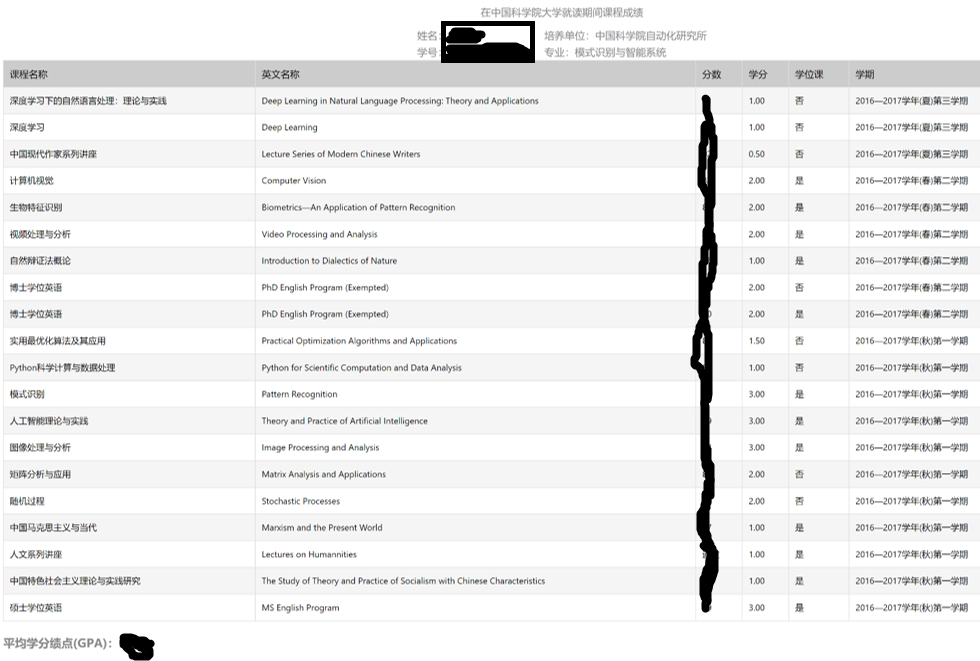
\includegraphics[width=0.99\linewidth]{Img/Others/score.png}
	\end{center}
	\caption{在中国科学院大学的已修课程和学分。
	}
	\label{fig:score}
\end{figure}
\begin{figure}[h]
	\begin{center}
		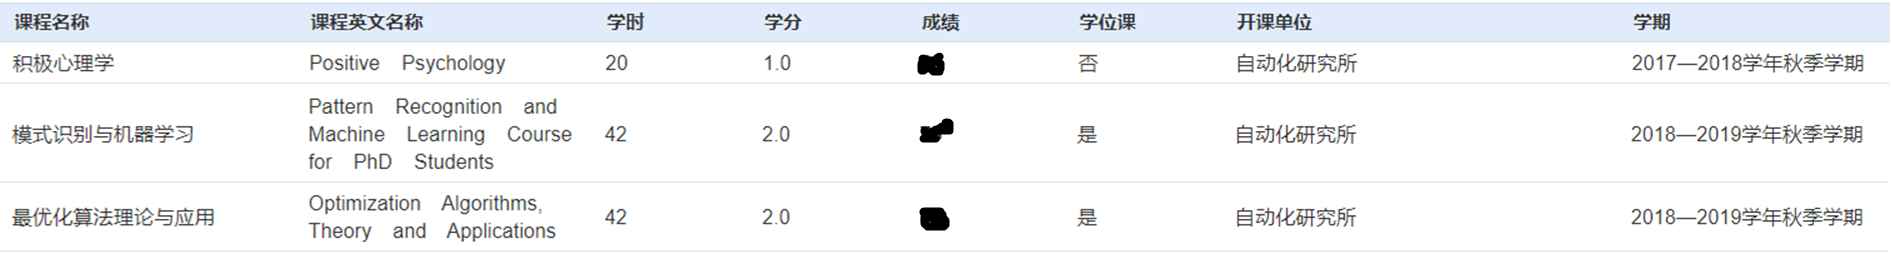
\includegraphics[width=0.99\linewidth]{Img/Others/score2.png}
	\end{center}
	\caption{在中国科学院自动化研究所的已修课程和学分。
	}
	\label{fig:score2}
\end{figure}

\chapter{学位论文开题存在的问题及回复}
学位论文开题时答辩老师主要关注的问题有两个。

一方面是xxx。回答如何解决。

另一方面是xxx。回答如何解决。

\chapter{学位论文撰写提纲}
\noindent 第一章\quad 绪论

介绍背景与意义,分析解决该任务存在的困难与挑战,并对本文的研究内容进行介绍。对学位论文的整体架构
进行描述。
\newline

\noindent 第二章\quad 国内外研究现状

介绍和本文相关的国内外研究现状。主要介绍xxx。
\newline

\noindent 第三章\quad 研究内容一

xxx。
\newline

\noindent 第四章\quad 研究内容二

xxx。
\newline

\noindent 第五章\quad 研究内容三

xxx。
\newline

\noindent 第六章\quad 总结与展望

xxx。